\begin{figure}
\centering
\begin{tikzpicture}
    \draw (0, 0) node[inner sep=0] {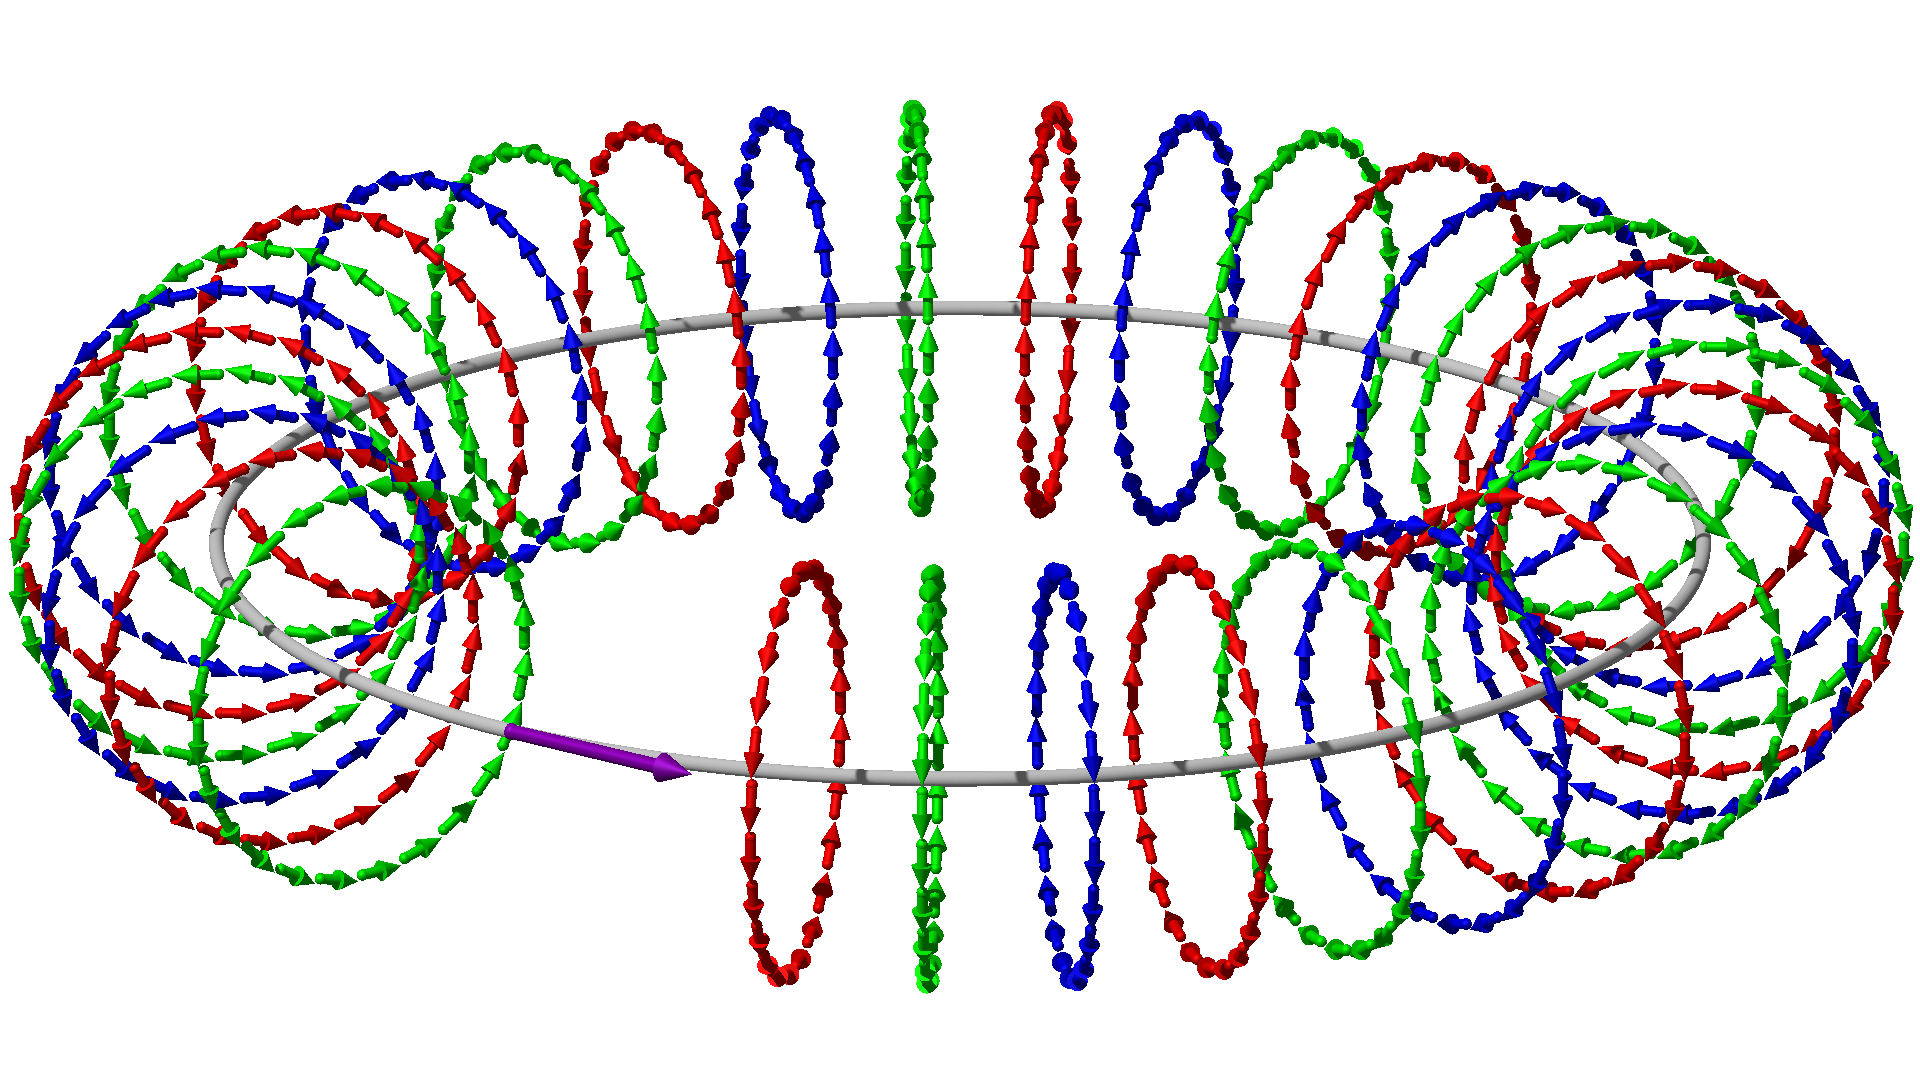
\includegraphics[width=1\textwidth]{papers/wirbelringe/fig/wirbelring_RGB.jpg}};
    \draw (-2.3, -1.05) node {\(\vec{\omega}\)};
\end{tikzpicture}
\caption{Typischer idealer Wirbelring.
Dargestellt durch momentane Bewegungsvektoren unterschiedlicher Teilchen in regelmässigem Abstand.
Zur besseren Übersicht sind Teilchen eines Wirbels mit derselben Farbe markiert.
Unterschiedliche, benachbarte Wirbel haben unterschiedliche Farben.
Die Wirbellinie ist als silbrige Linie eingezeichnet.
Ein einzelner Wirbelvektor \(\vec{\omega}\) ist violett in der Aussparung eingezeichnet.\label{Wirbelringe:fig:generell}}
\end{figure}